% Workshop short paper — Mechanical Verifiers as Objective Judges for Agent Reliability
% origin: ai · 2026-11-23 · 4 页单栏 (ICLR 2027 workshop track, 格式随各 CFP 微调)
% 源: workshop-draft-20261123.md (数字同源 data/, 精确一致)
% 编译: pdflatex (单栏, 10pt). 投具体 workshop 时换该 workshop 的 class 即可, 正文不变.
\documentclass[9pt]{article}
\usepackage[margin=1in]{geometry}
\usepackage{amsmath,amssymb}
\usepackage{graphicx}
\usepackage{subcaption}
\usepackage{booktabs}
\usepackage{hyperref}
\usepackage{xcolor}
\setlength{\parindent}{0em}
\setlength{\parskip}{3pt}
\setlength{\textfloatsep}{8pt}
\setlength{\floatsep}{8pt}

\title{Mechanical Verifiers as Objective Judges for Agent Reliability}
\author{Anonymous Submission}
\date{}

\begin{document}
\maketitle

\begin{abstract}
LLM judges are the default scorer in automated agent evaluation, but their reliability on the formalizable core --- where the correct answer is a numeric or spec-constrained quantity --- has not been measured against an exact reference. We measure it. On 67 real outputs from a 27b model across 10 tasks, a 27b LLM judge under three prompt variants fails to emit a parseable verdict on 52--84\% of checkpoints, and on the checkpoints it does parse, its verdicts disagree with a mechanical judge at $\approx$50\% --- indistinguishable from a coin flip (binomial $p = 0.79$--$0.90$). A mechanical judge (SymPy symbolic comparison or spec-driven regex) fails on 0/67 by construction. We isolate the mechanism: input complexity lengthens the judge's reasoning chain until it exhausts \texttt{max\_tokens} and truncates the verdict; raising \texttt{max\_tokens} recovers 3/6 truncated cases (the rest fail by chain non-convergence, not budget). We certify the task set against guessing via a model-agnostic bound ($P(\text{all-correct by guess}) \le 3.3\times10^{-5}$). On the formalizable core, a mechanical judge is exact, free, and reproducible --- and should be the default there.
\end{abstract}

\section{Why this matters}
Agent evaluation increasingly runs on LLM judges: automated pipelines score thousands of outputs per day, and the judge's reliability silently bounds the entire evaluation's validity. The reliability literature measures how wrong a judge is \emph{given that it emits a verdict} --- bias, position effects, self-preference --- but the upstream question, whether a parseable verdict is emitted at all, has not been measured against an exact reference. This matters because a judge that fails to parse on 52--84\% of checkpoints is not a noisy scorer; it is a scorer that is \emph{absent} on most of the data, and any aggregate reliability metric computed over the parseable subset is conditioned on a selection that the metric itself does not report. Our contribution is a measurement plus a mechanism plus a guarantee: we measure format reliability and verdict agreement on the formalizable core against a mechanical reference (F1, F3); we attribute the format failures to reasoning-chain truncation with direct engine evidence (F2, \S5); and we certify that the task set cannot be gamed by guessing (F4). The practical consequence: on the formalizable core, a mechanical judge is exact, free, and reproducible, and should be the default; the LLM judge belongs on the non-formalizable residual.

\section{Setup}
\textbf{Tasks.} 10 tasks (7 full-rank, 3 rank-deficient) over GPU systems and math/physics. Full-rank tasks have all parameters present and a unique answer --- e.g., ``given a 64-layer model with 8 KV heads and head dimension 128, compute the KV-cache bytes per token'' (gold: $64\cdot8\cdot128\cdot2$, tolerance 2\%). Rank-deficient tasks omit or conflict a key parameter, so the correct behavior is to report the gap rather than fabricate --- e.g., a memory-budget question that names the GPU SKU but omits its HBM capacity; the correct answer names the missing quantity, and a second checkpoint requires the still-computable total (weights + KV + overhead). Each task carries 4--5 checkpoints (47 total): calc checkpoints with a symbolic gold value and tolerance, and fact checkpoints anchored to vendor datasheets. Gold values are verified by SymPy self-check at construction time.

\textbf{Judges.} (i) LLM judge: the same 27b model (Qwen3-27B, vLLM, temperature 0) asked to verify a candidate answer under three prompt variants --- V1\_strict (JSON contract, exact values), V2\_loose (relaxed format), V3\_engineer (engineering-style rubric). (ii) Mechanical judge: SymPy symbolic comparison for calc checkpoints, spec-driven regex for boolean/fact checkpoints. The mechanical judge is exact on calc checkpoints by construction; on textual-gold checkpoints (naming a missing quantity) it is a regex heuristic and we report those separately.

\textbf{Protocol.} 67 real 27b outputs (7 full-rank $\times$ 1 + 3 rank-deficient $\times$ 10 reps per arm) $\times$ 3 prompt variants = 201 judge calls. \emph{Format reliability} = fraction of outputs the LLM judge fails to parse. \emph{Flip rate} = fraction of checkpoints (on parseable outputs, both judges verdicted) where the LLM verdict disagrees with the mechanical verdict.

\begin{figure}[t]
\centering
\begin{subfigure}[t]{\linewidth}
\centering
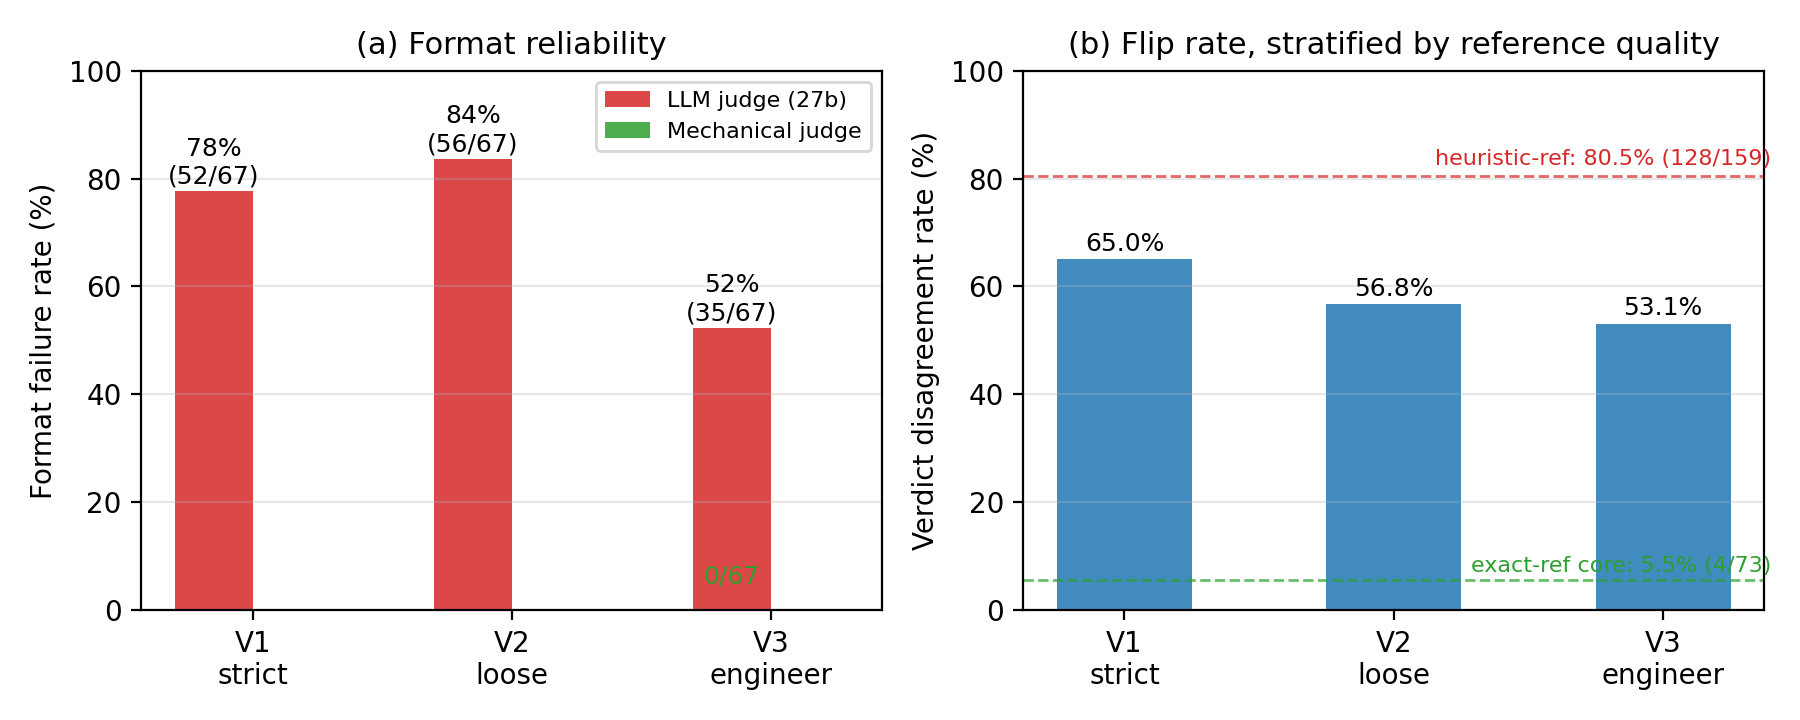
\includegraphics[width=0.85\linewidth]{figures/fig1-format-reliability.png}
\caption{Format failure rate (LLM vs mechanical judge) and flip rate on the parseable subset (dashed: 50\% coin flip).}
\label{fig:format}
\end{subfigure}
\begin{subfigure}[t]{\linewidth}
\centering
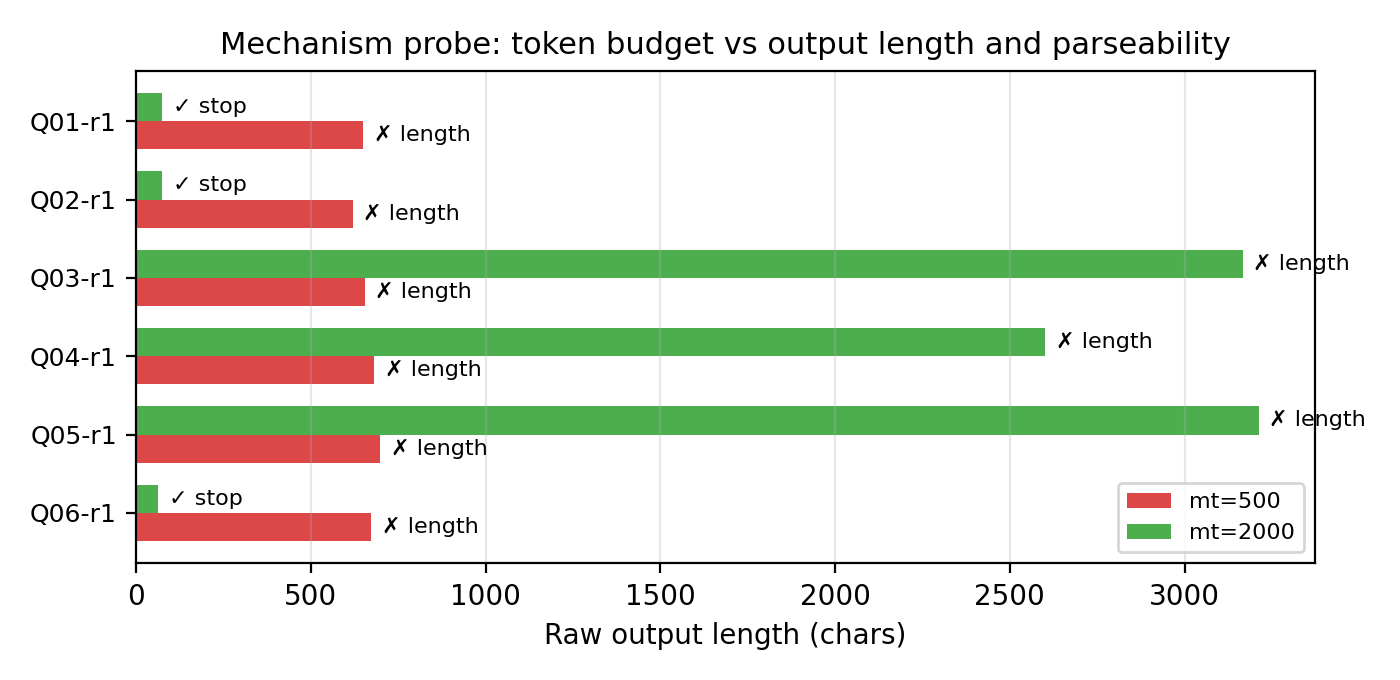
\includegraphics[width=0.85\linewidth]{figures/fig2-mechanism.png}
\caption{Mechanism probe: output length and parseability at \texttt{mt}=500 vs 2000 (recovered: Q01/Q02/Q06).}
\label{fig:mech}
\end{subfigure}
\caption{\textbf{(a)} Format reliability and verdict agreement under three prompt variants. \textbf{(b)} Token budget vs output length: raising \texttt{max\_tokens} recovers the short-verdict cases; non-converging chains (Q03/Q04/Q05) remain unparseable.}
\end{figure}

\section{Related work}
The LLM-as-a-judge reliability literature (a rapidly growing 2026 direction) measures judge \emph{bias} --- systematic deviations such as position, verbosity, and self-preference --- using human annotation or perturbation tests as ground truth. The closest six works: the Judge Reliability Harness \cite{judgeharness} stress-tests a judge against input perturbations (formatting, paraphrasing, label flip) but instruments input robustness, not the judge's own output format; Arena-Hard's judge analysis \cite{arenahard} varies judge model and rubric but assumes a verdict is emitted; Consistency $\neq$ Reliability \cite{consistency} shows self-consistency is not a reliability proxy, motivating our two-dimensional measurement; The Judge's Verdict \cite{verdict} analyzes judge capability against human labels on open-ended tasks; Metric Match \cite{metricmatch} selects evaluation subsets; VERA \cite{vera} conditions reliability on the emitted verdict. In the recursive-self-improvement track, TRUST \cite{trust} and three concurrent papers verify the \emph{agent being improved}; we verify the \emph{judge itself}.

Our differentiation is threefold. (a) \textbf{Format reliability}: prior work assumes the judge emits a score and measures how wrong it is; we measure the upstream failure --- the judge failing to emit a parseable verdict at all (52--84\%). (b) \textbf{Mechanism attribution}: prior work reports correlations (``reliability varies with X''); we attribute failures to an actionable mechanism (reasoning-chain truncation) with direct engine evidence (\texttt{finish\_reason=length}). (c) \textbf{Anti-guessing guarantee}: no prior work certifies that a high score is not achievable by guessing; we give a model-agnostic analytic bound.

\section{Findings}
\textbf{F1: Format reliability fails at 52--84\%.} \textbf{(Fig.~\ref{fig:format}a)} V1: 77.6\% (52/67, Wilson 95\% CI $[0.663, 0.859]$); V2: 83.6\% (56/67, $[0.729, 0.906]$); V3: 52.2\% (35/67, $[0.405, 0.637]$). The mechanical judge: 0/67. No prompt phrasing brings the LLM judge to usable format reliability; the best variant still fails over half of checkpoints. The failure is content-driven, not length-driven: full-rank tasks (complex symbolic gold) fail 7/7 across the full length range, while rank-deficient tasks (short gap-flagging responses) fail 45/60 with a length effect only within the group.

\textbf{F2: The mechanism is reasoning-chain truncation.} All six mt500 failure cases in the mechanism probe hit \texttt{finish\_reason=length} --- the token budget is exhausted before the JSON verdict begins. The causal chain unifies what earlier analyses reported as separate factors (truncation vs input complexity): \textbf{input complexity $\to$ longer reasoning chain $\to$ collision with \texttt{max\_tokens} $\to$ JSON truncated}. Input complexity is the upstream driver of chain length, not an independent additive factor.

\textbf{F3: Parseable verdicts flip at chance.} \textbf{(Fig.~\ref{fig:format}b)} V1: 31/60 (51.7\%, CI $[0.393, 0.638]$); V2: 21/44 (47.7\%, CI $[0.338, 0.621]$); V3: 66/128 (51.6\%, CI $[0.430, 0.600]$). Exact two-sided binomial tests against $p=0.5$ give $p=0.90$ (V1) and $p=0.79$ (V3); every CI contains 0.5. Scope: on the rank-deficient textual-gold checkpoints the mechanical reference is a heuristic (0/60), skewing flips toward LLM-correct; excluding them the flip rate is V1 27/45 (60.0\%), V2 17/33 (51.5\%), V3 45/96 (46.9\%) --- still $\approx$50\% everywhere. The coin-flip claim rests on calc-gold checkpoints, where the reference is exact.

\textbf{F4: The task set is not guessable.} We define a random-guess model (independent sampling per checkpoint type: $U[0.5g, 2g]$ for continuous calc, $U\{g\pm50\}$ for integer-exact, $1/100$ for textual gold) and derive an analytic upper bound on $P(\text{all checkpoints correct by guess})$: full-rank $1.2\times10^{-10}$ to $1.9\times10^{-7}$; rank-deficient $3.6\times10^{-6}$ to $3.3\times10^{-5}$ (highest: fewer checkpoints + textual gold). Monte Carlo ($N=2000$, seed=42): 0/2000 all-correct, consistent with the bound. The bound is conservative (independence assumption, $1/100$ textual constant) --- high scores on this set are not achievable by guessing, and the bound is model-agnostic.

\textbf{F5: Prompt optimization trades dimensions.} The rank-deficient arms (A\_baseline / B\_remind / B'\_remind, $n=10$ per arm $\times$ 3 questions = 30 outputs) show the trade: B\_remind fixes c1 (10/30 $\to$ 30/30) but degrades c4 (30/30 $\to$ 21/30); B'\_remind fixes c1 (10/30 $\to$ 30/30) and keeps c4 at 30/30 but c3-strict drops 25/30 $\to$ 23/30. The 7/30 gray-zone cases (all Q08, B' arm) are conditional enumerations --- the B' prompt \emph{induces} hedging behavior (``if 64 GB then\ldots if 80 GB then\ldots''), a behavioral-level signature of the prompt effect: strict scoring marks these as miss (no single committed value), lenient scoring (hedging-word exemption) marks them pass (30/30). No arm is 100\% on all dimensions: prompt engineering on the judge moves failure between checkpoint dimensions rather than eliminating it.

\section{Mechanism: truncation, and the self-repair case}
\textbf{(Fig.~\ref{fig:mech})} Raising \texttt{max\_tokens} 500$\to$2000 recovers 3/6 cases (Q01/Q02/Q06 emit short pure-JSON verdicts, 63--74 chars); the three non-recoveries (Q03/Q04/Q05) emit 2600--3200-char reasoning chains that cycle without converging --- recovery is determined by whether the reasoning chain converges, not by \texttt{max\_tokens} itself. The same input at temperature 0 flips between parseable and unparseable across runs (Q04: 3/5), so format reliability is not merely low, it is \emph{unstable}. The root cause is instruction-following non-determinism at temperature 0: obeying ``output JSON only'' $\to$ short output $\to$ parseable; disobeying $\to$ long reasoning chain $\to$ truncation (at mt500) or cycling (at mt2000).

\textbf{Self-repair case.} Q01 at mt500: the judge's reasoning chain exhausts 500 tokens mid-derivation, no verdict emitted (unparseable, 0/5 runs). Same input at mt2000: the chain converges, the judge emits a 74-char pure-JSON verdict with all checkpoints correct (5/5 runs, deterministic). The failure is a budget artifact, not a capability gap --- which is exactly why the mechanical reference (which has no reasoning chain to truncate) is the appropriate default on the formalizable core.

\section{Implications and limitations}
\textbf{Implications.} (i) On the formalizable core, use the mechanical judge: free, 100\% reliable on calc checkpoints, reproducible. (ii) Reserve LLM judgment for the non-formalizable residual (explanation quality, argument structure). (iii) Harness design: \texttt{max\_tokens} must exceed the P99 of the judge's output-length distribution, and JSON-only decoding removes the truncation failure mode. (iv) Benchmark design: checkpoint count is not the anti-guessing lever --- gold complexity is (F4). (v) The convergence-failure cases (Q03/Q05) fail even at mt2000, so a non-zero failure floor remains under any budget; the mechanism (reasoning-chain exhaustion) is the robust claim, the exact rates are budget-dependent.

\textbf{Limitations.} Single model (27b), single task set (10 tasks); cross-model generalization untested. \texttt{max\_tokens}=500 is the default configuration; production deployments may differ. Rank-deficient tasks number 3. The textual-gold checkpoints rely on a regex heuristic reference, reported separately (F3 scope note). The v1$\to$v2 mechanism-probe discrepancy (Q04/Q05 recovery flags) is a temperature-0 run-to-run flip, recorded for transparency in the full version.



\begin{thebibliography}{9}
\footnotesize
\setlength{\itemsep}{1pt}
\bibitem[judgeharness]{judgeharness} Dev et al. 2026. Judge Reliability Harness. arXiv:2603.05399.
\bibitem[arenahard]{arenahard} Behind Aggregate Scores: Arena-Hard judge analysis. arXiv:2610.30512.
\bibitem[consistency]{consistency} When Consistency Does Not Mean Reliability. arXiv:2609.13824.
\bibitem[verdict]{verdict} The Judge's Verdict. arXiv:2510.09738.
\bibitem[metricmatch]{metricmatch} Metric Match. arXiv:2606.15029.
\bibitem[vera]{vera} VERA. arXiv:2610.05452.
\bibitem[trust]{trust} TRUST. arXiv:2611.10787 (under review ICLR 2027).
\end{thebibliography}

\end{document}
